\newpage
\part{Rendu}
    Après avoir détecter le tag dans l'image, la seconde grande étape est de projeter un modèle 3D sur la scène. Pour cela, l'utilisateur indique au lancement du programme le ou les modèles à utiliser, avec ou non des matériaux, et ceux-ci seront rendus à chaque image.

    \section{Gestion des objets}

        \subsection{Objets}

            \subsubsection{Définition du format}                
                Un objet 3D est composé de sommets, formant des faces d'au moins 3 côtés. Le format le plus simple pour stocker un modèle 3D est le \emph{.obj}. Cette norme définie les sommets, les matériaux et les normales pour chaque face dans un format texte. Chaque ligne début par un indicateur puis les valeurs à proprement parler. Un exemple est visible figure \ref{fig:obj}. Nous utilisons 4 indicateurs :
                \begin{itemize}
                    \item v x y z : sommet à la position $(x, y, z)$
                    \item vt u v [z] : coordonnées de texture (voir partie \ref{subsubsec:materiaux})
                    \item vn x y z : normale (voir partie \ref{subsubsec:lumiere})
                    \item f v/vt/vn [...] : les faces de l'objet avec un triplet pour chaque sommet (minimum 3). La coordonnée de texture peut être vide (v//vn).
                \end{itemize}
                
                \begin{figure}[h]
                    \centering
                    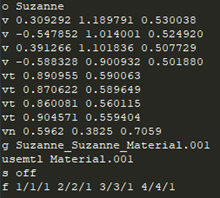
\includegraphics[scale=0.8]{img/rendu/obj.png}
                    \caption{Exemple de fichier \emph{.obj}}
                    \label{fig:obj}
                \end{figure}
                Nous avons écrit un parser afin de décomposer ce fichier \emph{.obj}.

                Chaque objet est contenu dans une classe \emph{Object}. Celle-ci contient un ensemble de face qui correspond à plusieurs points, une couleur et une normale. Plusieurs fonctions sont également disponible afin de manipuler l'objet : \emph{rotate}, \emph{scale}, \emph{position}\dots

            \subsubsection{Matériaux}
            \label{subsubsec:materiaux}

            Afin de rendre les objets plus agréables à l'\oe il, nous avons décider d'implémenter la gestion des matériaux. Nous utilisions déjà le format \emph{.obj} pour les modèles, il semblait donc naturel d'utiliser les \emph{.mtl}, format défini par la même norme, pour les matériaux. 

            Un fichier \emph{.mtl} est un fichier texte, et nous utilisons uniquement une seule ligne de ce fichier, \emph{map\_kD}, qui indique le nom de l'image texture utilisée. Les coordonnées de texture renseignées dans le \emph{.obj} indiquent des pourcentage dans cette image, respectivement la largeur et la hauteur. Nous travaillons ici avec des images 2D.

            \begin{figure}[h]
                \centering
                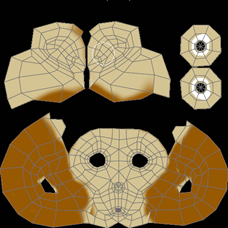
\includegraphics[scale=0.8]{img/rendu/texture.png}
                \caption{Texture découpée par face}
                \label{fig:texture}
            \end{figure}

            Dans la figure \ref{fig:texture}, nous pouvons voir les faces en fonction des coordonnées indiquées pour chaque sommet. Afin de pouvoir utiliser cette texture, il faut déformer le polygone pour l'appliquer sur le polygone projeté. Cependant, cette étape est très coûteuse en performance car il faut l'appliquer pour chaque polygone de chaque objet à chaque image de la vidéo. Nous avons alors choisi de préférer le temps réel et, pour cela, une face ne possède qu'une seule couleur, inscrite directement dans la classe \emph{Object}. Pour choisir la couleur, nous prenons simplement la couleur du pixel au centre du polygone sur l'image texture. Cela nous donne alors un objet avec des flat color. 
            
            Une amélioration possible du programme pourrait être de prendre en compte les autres paramètres du fichier \emph{.mtl} et donc de ne pas obligatoirement utiliser d'image pour la texture.

        \subsection{Scène}

        La scène contiendra tous les objets 


        \subsection{Lumière}
        \label{subsubsec:lumiere}

        Une méthode d'ombrage plat (\textit{Flat Shading}) a été implémentée afin de rendre l'apparence des objets plus réaliste.

        La lumière est représentée par un vecteur qui donne sa direction. La luminosité d'une face de l'objet est calculée en fonction de l'angle entre sa normale et la direction de la lumière.

        \begin{figure}[!h]
            \centering
            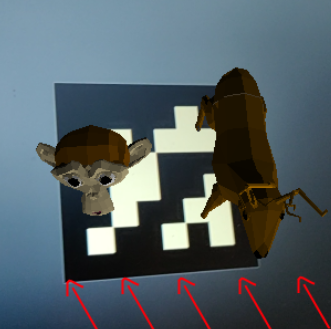
\includegraphics[scale=0.5]{img/flat_shading.png}
            \caption{Ombrage plat sur les objets à partir d'une source lumineuse représentée par les flèches rouges}
        \end{figure}

    \section{Projection et caméra}

        \subsection{Calibration}
        
        \subsection{Projection}
        % TODO: expliquer l'extraction de z via l'homographie
